\documentclass[letterpaper,twocolumn,10pt]{article}
\usepackage{usenix2019_v3}

\usepackage{tikz}
\usepackage{amsmath}
\usepackage{amssymb}
\usepackage{pifont}
\usepackage{comment}

\newcommand{\cmark}{\ding{51}}
\newcommand{\xmark}{\ding{55}}

\usepackage{graphicx}
\usepackage{hyperref}
\usepackage{float}
\usepackage{listings}
\usepackage{booktabs}
\usepackage{paralist}
\usepackage{titlesec}

\titleformat*{\subsection}{\normalsize\bfseries}
\titleformat*{\subsubsection}{\normalsize\bfseries}
\titlespacing{\subsection}{0pt}{1ex}{0.5ex}
\titlespacing{\subsubsection}{0pt}{0.5ex}{0ex}

\begin{document}
\newcommand{\twosigma}{[tech company]} 
\date{}
\title{\Large \bf DRAFT: Direct-style process creation on Linux}
% \author{
% {\rm Spencer Baugh}\\
% Two Sigma
% }
\maketitle
\begin{abstract}
Traditional process creation interfaces,
such as fork and spawn,
are complex to use, limited in power, and difficult to abstract over.
We develop a new process creation interface for Linux
which allows a program to create a child process in an non-running state
and initialize the new process by operating on it from the outside.
This method of process creation results in more comprehensible programs, 
has better error handling,
is more efficient,
and is more amenable to abstraction.
Our implementation is immediately deployable without kernel modifications on any recent Linux kernel version.
\end{abstract}

\section{Introduction}\label{introduction}
Existing process creation interfaces can be divided into three categories:
Fork-style, spawn-style, and direct-style.

Fork-style (such as \texttt{fork}) and spawn-style (such as \texttt{posix\_spawn}) are the most popular,
but have a number of disadvantages.
Correct, performant use of fork-style places significant constraints on the calling process,
and also has a complex programming model.
Spawn-style lifts many of these constraints, and is simpler to program against,
but is fundamentally limited in the kinds of processes it can create.
With both fork-style and spawn-style,
it is difficult to
branch based on results or errors encountered while initializing the new process:
fork-style requires IPC if it wishes to communicate errors back to the rest of the program,
and robust indication of errors in spawn-style requires substantial expansion of the spawn interface.

Direct-style is more rarely seen, but gives a number of advantages.
Direct-style involves creating a new child process in a non-running state,
and then calling individual system calls from the parent to initialize the child.
Direct-style does not constrain the calling process,
easily branches at any step of the initialization,
and can create any kind of process supported by the underlying system.

Our contribution is an implementation of direct-style process creation for Linux,
making use of our work on the \texttt{rsyscall} project.
The \texttt{rsyscall} project develops language-specific ``process-independent'' system call libraries for Linux,
which replace libc system call wrappers,
and allow a program to perform cross-process system calls.
\texttt{rsyscall} works entirely in userspace
and can be deployed on existing Linux systems without kernel modifications.
\texttt{rsyscall} is currently focused on supporting, and is implemented in, Python,
but can be ported to other languages;
the examples we show in this paper will be in Python,
but generalize easily to other languages.

Our direct-style process creation implementation uses \texttt{clone} to create a child process in an embryonic state
which can then be manipulated from user code in the parent process using syscalls with \texttt{rsyscall}.
A direct-style \texttt{clone} has all the advantages of direct-style process creation
over Linux's fork-style \texttt{fork} and spawn-style \texttt{posix\_spawn}:
\begin{compactitem}
\item
  Processes can be created correctly and performantly from any parent process,
  with a straightforward, familiar API.
\item
  Processes can be created with the full set of Linux features.
\item
  Syscall results are reported individually to the parent process.
  % rather than batched together as with spawn-style or manually reported via IPC as with fork-style.
\end{compactitem}

We've implemented a variety of useful applications using direct-style process creation on Linux,
which we'll demonstrate in this paper.
Direct-style \texttt{clone} has minimal performance cost in normal situations,
and can outperform \texttt{fork} in some cases.
We have deployed direct-style process creation in production internally at \twosigma.

Our implementation is distributed as a feature of \texttt{rsyscall},
and is immediately deployable, entirely in userspace, on recent Linux kernels.
\texttt{rsyscall} is open source and available from
[Github url].
% \url{https://github.com/catern/rsyscall}.

This paper is organized in several sections.
\begin{compactitem}
\item Section \ref{background} provides background on fork-style, spawn-style, and direct-style process creation,
and considers their advantages and disadvantages in more depth.
\item Section \ref{overview} discusses the design of the API,
including our usage of \texttt{rsyscall}.
\item Section \ref{examples} shows examples of direct-style process creation in Python on Linux,
including use of process features which are difficult to use on Linux with \texttt{fork} or \texttt{posix\_spawn}.
\item Section \ref{implementation} explores our implementation in depth,
and discusses several difficult process-creation related details of \texttt{rsyscall}.'s implementation.
\item Section \ref{evaluation} evaluates our results using both quantitative and qualitative approaches.
\item Section \ref{related_work} examines other work which also touches on the topics covered by this paper.
\item Section \ref{future_work} lists several directions for future work
related to direct-style process creation and to \texttt{rsyscall}.
\item Section \ref{conclusions} briefly outlines our conclusions about direct-style and the future of process creation.
\end{compactitem}
\section{Background on process-creation}\label{background}
As mentioned in the introduction,
on most operating systems today,
the available interfaces for process creation
are either "fork-style" or "spawn-style".
A few operating systems have a third style, which we refer to as "direct-style".

% Ugh, these aren't the same size right now.
\newcommand{\tbad}{\xmark:}
\newcommand{\tgood}{\cmark:}
% \newcommand{\tbad}{\text{\sffamily X} :}
% \newcommand{\tgood}{\checkmark:}

\begin{table*}
\begin{tabular}{l|l|l|l}
% BEGIN RECEIVE ORGTBL compare
 & fork-style & spawn-style & direct-style\\
\hline
Works with any caller & \tbad No threads or large memory & \tgood Yes & \tgood Yes\\
Programming model & \tbad Complex (returns twice) & \tgood Simple (single call) & \tgood Simple (imperative)\\
Maximally powerful & \tgood Yes, can call any syscall & \tbad No, limited interface & \tgood Can call any syscall\\
Error handling & \tbad Poor, requires IPC & \tbad Poor, not fine-grained & \tgood Reports individual errors\\
Non-copied attributes & Mutated by code in child & Set by arguments & Mutated by code in parent\\
% END RECEIVE ORGTBL compare
\end{tabular}
\caption{Features of fork-style vs spawn-style vs direct-style}
\label{tab:ease}
\end{table*}
\begin{comment}
#+ORGTBL: SEND compare orgtbl-to-latex :splice t
|                       | fork-style                       | spawn-style                  | direct-style                     |
|-----------------------+----------------------------------+------------------------------+----------------------------------|
| Works with any caller | \tbad No threads or large memory | \tgood Yes                   | \tgood Yes                       |
| Programming model     | \tbad Complex (returns twice)    | \tgood Simple (single call)  | \tgood Simple (imperative)       |
| Maximally powerful    | \tgood Yes, can call any syscall | \tbad No, limited interface  | \tgood Can call any syscall      |
| Error handling        | \tbad Poor, requires IPC         | \tbad Poor, not fine-grained | \tgood Reports individual errors |
| Non-copied attributes | Mutated by code in child         | Set by arguments             | Mutated by code in parent        |
% $
\end{comment}
\subsection{Fork-style}
By far the most well-known fork-style interface is Unix's fork.\cite{forkhist}
With a fork-style interface,
a process, called the parent process, calls \texttt{fork},
and a copy of that process is made,
called the child process,
differing only in a few attributes such as process id.
The same program continues executing in both processes,
with a different return value from fork to allow it to distinguish whether it is running in the parent or the child.
Typically, the program will branch based on the return value
and, if running in the child,
call various system calls to modify the state of the new process.

Fork has a number of flaws,
and much ink has been spilled detailing them.
We'll cover the most egregious briefly here,
but see Baumann 2019 \cite{forkroad} for a more detailed evaluation.

Fork, when called successfully, returns twice,
creating two different processes which execute concurrently.
This immediately makes fork difficult to integrate;
for example, errors can't be easily communicated between the two processes.
If there is an error in the initialization of the child process,
the part of the program running in the child process
needs to use some form of inter-process communication (IPC) to communicate it back to the parent process.
The child process can run arbitrary code to make decisions about its initialization,
but that code needs to use IPC if it wishes to communicate with the rest of the program,
which is still in the parent process.

Fork can have poor performance when called from processes with many memory mappings.\cite{forkroad}
Fork copies many attributes about the parent process when creating the child process,
including setting up copy-on-write memory mappings in the child process.
This becomes slower as the parent process has more memory mappings,
eventually taking a significant amount of time.
This copying is required to robustly implement fork's model,
where the same program continues executing without changes in both the parent process and child process;
the copy of the program running in the child process might access any memory at any time.

Multi-threaded programs generally cannot use fork safely.
Typical Unix fork implementations duplicate only the thread calling fork from the parent process to the child process.
In a multi-threaded program, this can cause various issues;
for example, another thread might be holding a memory allocator lock at the time of the fork,
which in the child process will never be unlocked,
causing the child process to deadlock if it tries to allocate memory.
Some thread libraries provide partial mitigations for this issue,
but it's up to user code to make use of those mitigations.\cite{pthread_atfork}
In combination with fork's poor performance in large-memory programs,
a user of fork must think carefully
about the characteristics of the process from which fork is being called.
\subsection{Spawn-style}
In a spawn-style interface,
details about the new process are provided up-front as arguments to some function
which creates the new process all at once.
The most well known spawn-style interfaces are Unix's \texttt{posix\_spawn} \cite{posix_spawn}
and Windows \texttt{CreateProcess} \cite{create_process};
the Unix shell also serves as a spawn-style process creation interface,
especially when used with Bernstein chaining\cite{chainloading}.

Spawn-style interfaces typically still transparently copy some details from the parent process;
for example, various security contexts,
and any other process attribute which is not explicitly specified in the arguments to the spawn interface.
The key difference between fork-style and spawn-style is not how much they copy,
it is how the attributes which are not copied are specified:
by mutation from code running in the new process in the case of fork-style,
or by explicit argument passing in the case of spawn-style.

Spawn-style interfaces lift the constraints on the calling process that fork-style interfaces impose.
Spawn-style interfaces don't run user code in the new process during initialization.
This means there is no need to copy memory,
so performance is good when a spawn-style interface is used from a process with many memory mappings.
Likewise, there are no inherent issues when a spawn-style interface is used from a multi-threaded program,
though operating systems, such as Linux,
which implement spawn-style interfaces on top of \texttt{fork} can still have threading bugs.

The arguments that can be provided to a spawn-style process creation syscall
do not cover all the possible attributes that one might want to set for the new process.
Most systems have a large number of syscalls which can mutate the state of a process during its lifetime;
for a spawn-style interface to work in all scenarios,
all those possible mutations must be reproduced in the interface.
For example, the \texttt{posix\_spawn} function provided by glibc does not support creating processes in new namespaces,
as is required for container functionality on Linux.

Spawn-style process creation
essentially creates a new domain-specific language for specifying the attributes of the process.
Fork-style allows existing system calls,
with which programmers are already familiar,
to be used to set up the new process.
Spawn-style requires some form of declarative description of the new process,
which must be learned in addition to the normal system call interface.

Spawn-style process creation also does not allow for conditional logic during the setup.
If the setup of the new process encounters an error at some point,
the only option is to return from the entire spawn call with an error.
Such errors returned from spawn-style calls
are typically much less informative
than the errors returned by the syscalls which directly mutate the process attributes.
Other forms of conditional logic are also impossible in spawn-style;
one modification to the process cannot depend on the result of some other modification.
\subsection{Direct-style}
A few academic operating systems, such as KeyKOS \cite{keykos}, seL4 \cite{sel4}
and some others \cite{exokernel} \cite{fuschia} \cite{singularity},
use another style of process creation.
We use the new term "direct-style" to refer to this,
since we know of no pre-existing concise and generic term for this style of process creation.

In direct-style, a process is created by its parent in a non-running state,
then supplied with various resources,
and then started running once it is fully set up.
In operating systems with true direct-style process creation,
the syscalls that can mutate a process
take explicit arguments to indicate the process on which they should operate.
In this way, the same syscalls that can mutate a process while it is running
are called by the parent process to mutate the process while it is being set up.

We refer to this as "direct-style" process creation,
because the parent creating the process operates on it directly and imperatively
rather than dispatching a distinct unit of code to perform setup from inside the context of the new process,
as in fork-style,
or building up a declarative specification of what the new process should look like ahead of time,
as in spawn-style.

Since everything happens directly from the parent process,
direct-style process creation is compatible with a variety of techniques
which are difficult with fork-style or spawn-style.
For example, a REPL could be used to interactively create the new process,
or a program might initialize several processes at once and share data between them.

Significantly,
since all operations are performed through syscalls called directly from the main program,
errors are indicated in the same way as any other syscall error.
This is unlike fork-style, which needs IPC to indicate errors,
and unlike spawn-style, which typically indicates errors at a very coarse-grained level.

Like fork-style interfaces,
direct-style interfaces can set up arbitrary attributes in the new process.
Any attribute that can be changed by a syscall
can be manipulated by a direct-style interface,
just as with fork-style interfaces.
This is unlike spawn-style interaces,
which only can change attributes that are supported by the interface.

Like spawn-style interfaces,
direct-style interfaces have no constraints on the calling process.
Also like spawn-style interface,
no user code runs in the child process, so
direct-style interfaces can be used from multi-threaded or large-memory processes without issues.

Direct-style can be more complex to use;
it is most typically used in capability-oriented operating systems,
where a great deal of resources and information must be provided explicitly to initialize the new process.
In a truly capability-oriented operating system,
nothing is copied implicitly to the new process;
everything must be explicitly specified.
This can appear more complex
when compared to process creation on Unix systems or Windows.

However, we believe that a natural port of direct-style process creation to Linux
provides an interface that is just as simple to use as fork-style or spawn-style on Linux,
without their disadvantages.
Such an interface, like fork-style and spawn-style,
would implicitly copy some attributes to the new process,
rather than being capability-oriented and requiring all attributes to be specified explicitly.
This is the kind of direct-style interface that we contribute in this paper.
\section{Overview of API}\label{overview}
In most operating system APIs, including the ones available on Linux,
when a program makes a syscall, it implicitly operates on the current process.
To perform direct-style process creation on Linux,
we need an API where we instead explicitly specify in which process we want to make a syscall.

\texttt{rsyscall} provides this API.
The \texttt{rsyscall} project develops
language-specific, object-capability-model, low-abstraction libraries for the Linux syscall interface,
bypassing libc.

Unlike POSIX C libraries such as glibc or musl,
an \texttt{rsyscall} library is organized based on the object-capability model.
The capabilities to make syscalls in any given process are reified as language objects.
If the capability to make syscalls in a specific process is not passed (in some way) to a function,
then that function cannot make syscalls in that process.

Due to this design, an \texttt{rsyscall} program can make use of multiple processes at once,
by manipulating capabilities for multiple processes.
The relevant two capabilities for this paper are the initial capability to the ``local'' process,
and capabilities to child processes.
The ``local'' process is the one which hosts the runtime for the running program,
and in which a legacy libc would implicitly make syscalls.
Every \texttt{rsyscall} program starts with the ``local'' process
and uses it to bootstrap the initial capabilities for other processes.

To perform direct-style process creation,
we use \texttt{rsyscall} to call \texttt{clone} on the ``local'' process to create a new child process.
We call various syscalls in the child process to mutate it until it reaches the desired state,
at which point we can call \texttt{execve} in the child process to start it running on its own.
After that, the process is no longer under our control, and it functions like any other child process.
The child process can be monitored using normal Linux child monitoring syscalls,
such as \texttt{waitid}.

\lstinputlisting[float=ht,language=Python,label={basic},caption={Creating a new process, changing CWD, and execing}]
{examples/basic/direct.py}
Listing \ref{basic} shows this in action in Python.
We create a new child process using \texttt{clone} on the local process \verb|local|,
and receive back a capability to control it.
We call \texttt{chdir} in the child process to change its working directory to \texttt{/dev}.
Then we call \texttt{execve} in the child,
passing the path of the \texttt{cat} executable,
the arguments to the new executable,
and the unchanged set of environment variables.
The name of the executable is passed as the first argument,
as is typical in Unix.
Calling \texttt{execve} consumes the capability,
and later use of this child process capability will fail with an exception.

The behavior of system calls made on a remote process through \texttt{rsyscall}
is identical to the behavior of system calls made implicitly on the current process through libc.
This is an API that systems programmers are already familiar with,
and which is already thoroughly documented through Linux system call manpages.
The novelty is constrained to the newly explicit process capabilities.

The lack of novelty in the API is important not only for the learning curve,
but also for power.
Since we are using conventional Linux system calls,
just in a cross-process way,
direct-style \texttt{clone} will always be at least as powerful as \texttt{fork}.
\section{Examples}\label{examples}
In this section,
we'll demonstrate direct-style process creation
by demonstrating several advanced uses of processes
using more sophisticated Linux features.
For concision, we assume in these examples that we are running with sufficient permissions in these examples,
but these examples can all be run without privileges with appropriate use of \verb|CLONE_NEWUSER|.

These examples are not novel, as such, as they use only conventional Linux system calls;
but implementing them with \texttt{fork} or \verb|posix_spawn| requires substantially more code,
or even a complete change in implementation approach,
as described in section \ref{shared_fd_table}.
We'll compare our direct-style implementations in this section
to fork-style implementations
in section \ref{evaluation}.

Several of these examples provide functionality that can be done today by specialized software and services.
Such software often enables one or two of these uses of processes, but prevents others.
For example, a shell allows the creation of pipelines and container systems like Docker allow sandboxing,
but the two are difficult to combine.\cite{docker_pipe}

One of the key advantages of direct-style process creation is that the features we demonstrate here
can be easily used in combination,
to meet the specific needs of individual real-world applications.
\subsection{Abstraction through file descriptor passing}\label{fd_abstraction}
In Linux (and Unix in general),
a program can pass file descriptors from the parent process to a child process
by using file descriptor inheritance.
All open file descriptors are copied at process creation time from the parent process to the child process;
the child process can then make independent use of the file descriptors.
We'll discuss this important feature further in section \ref{fdtables}.

% TODO need to clarify this more, this is v2, Larry didn't like v1 beyond first sentence
Most resources in Linux are managed through file descriptors,
so this feature allows the parent process to pass a variety of resources to the child process,
such as files, network connections, pipes, or other resources.\cite{ucspi}
Since the resource is created outside the child process and passed down as an opqaue file descriptor,
the precise details and type of the resource are not available to the child.
This is a form of abstraction,
and we can know ``for free''\cite{theoremsforfree}
that the program running in the child process
will not rely on the details of how the file descriptor was created,
such as the filename that was opened or the hostname that was connected to.

\lstinputlisting[float=*ht,language=Python,label={fds},caption={Passing down FDs}]
{examples/fds/direct.py}
In Listing \ref{fds},
we first open a file with read-write permission in the local process.
Then we create a child process,
which inherits all file descriptors from its parent.
We indicate that we want to operate on the child's inherited copy of the file descriptor with \verb|child.inherit_fd|.
Then we disable \texttt{CLOEXEC} on the child's file descriptor,
which on Linux we can do by clearing the FD flags with \verb|fcntl(fd, F_SETFD, 0)|.
Finally, we execute some executable in the child process,
passing the file descriptor number as an argument;
since we disabled \texttt{CLOEXEC} on the file descriptor,
the executable will be able to use that file descriptor through that file descriptor number.
Unlike in listing \ref{basic}, we call the \texttt{execv} wrapper rather than \texttt{execve},
so that we don't need to pass the (unmodified) environment to every \texttt{exec} call in these examples.
\subsection{Non-shared-memory concurrency}
Processes run concurrently,
which allows exploiting the parallelism of the underlying hardware.
Since processes don't share memory,
they can provide a less complex parallel programming environment
than shared-memory thread-based approaches.

One of the most popular parallel programming environments is the Unix shell,
which obtains its parallelism by running multiple processes connected via pipes.
The Unix shell has a relatively constrained form of parallel processing,
but it's also possible to create more complex webs of parallel processes,
where, for example, one process might take multiple inputs over multiple pipes,
or produce multiple outputs.

\lstinputlisting[float=*ht,language=Python,label={pipe},caption={Creating a parallel processing pipeline}]
{examples/pipe/direct.py}
In listing \ref{pipe},
we execute a few programs in parallel,
connected by pipes.
We first create two pipes in the local process,
then inherit them down to several child processes using a helper function, \verb|as_argument|,
which uses \verb|inherit_fd| and \texttt{fcntl} as described in section \ref{fd_abstraction}.
We call exec in each child process, passing some file descriptors as arguments to the new programs.
The whole system then runs in parallel,
as normal child processes.
\subsection{Customization without explicit support}
While, ideally, all resources would be passed by file descriptor\cite{capsicum},
Unix has a number of resources that are global,
such as the pid space or the mount table,
and which cannot be changed on a per-process basis.

In Linux, most global resources have been made process-local
through the namespaces system.
Like other process-local resources such as the current working directory,
namespaces are typically set up at process creation time.

The most popular usage of namespaces is for large-scale container systems such as Docker;
however, this is far from the only use.
With an adaquate process creation primitive,
namespaces can be used easily on a much smaller scale.

Namespaces, like all process-local resources,
can be used to customize a program's behavior
in ways that were not anticipated at development time
by customizing the environment the process runs in.
Other system calls such as \texttt{chroot} can also be used for this.

\lstinputlisting[float=*ht,language=Python,label={mount},caption={Overriding absolute path using a mount namespace}]
{examples/mount/direct.py}
One classic form of customization enabled by namespaces
is overriding files at paths that were hardcoded into a program we can't change,
without changing those files for the rest of the system.
In listing \ref{mount},
we create a new child process as normal,
but for the first time,
pass an argument to \texttt{clone}.

\verb|CLONE_NEWNS| causes clone to create the process in a new mount namespace,
which allows us to manipulate the filesystem tree in a way that only this process will see
using the \texttt{mount} system call.
We call \texttt{mount}, passing \texttt{MS.BIND}, to make the file \verb|/home/foo/custom_foo.conf|
appear at the path \verb|/etc/foo.conf|.
This is known as a bind mount.
Then we execute some executable,
which, when it opens \verb|/etc/foo.conf|, will see the contents of our \verb|custom_foo.conf|.
\subsection{Sandboxing}
At process creation time,
we can not only pass resources and customize the process's environment,
we can also deny the process access to resources that it otherwise receives by default.
This is a key part of creating a secure sandbox for potentially malicious code.

\lstinputlisting[float=*ht,language=Python,label={unmount},caption={Unmount all and run executable via fexec}]
{examples/unmount/direct.py}
In listing \ref{unmount}
we create a new child process,
again in a new mount namespace using \verb|CLONE_NEWNS|.
We open the executable that we'll later exec in this child process,
as well as another file as in listing \ref{fds},
since we won't be able to do exec or open files normally after the next step.
Then we use \texttt{umount},
passing \texttt{MNT.DETACH} to perform a recursive unmount of the entire filesystem tree,
removing it all from the view of this process.
As in listing \ref{fds}, we unset the \texttt{CLOEXEC} flag from the database file descriptor,
so that it can be inherited across \texttt{exec};
we don't need to call \verb|inherit_fd| since, in this case, the database fd was opened directly from the child.

We then exec the file we opened earlier, using \texttt{fexec},
which allows execing a file descriptor,
and also pass the database file descriptor as an argument,
as in listing \ref{fds}.
(The underlying system call for \texttt{fexec} is \texttt{execveat};
this \texttt{fexec} is a helper function.)
Note that this executable must be statically linked,
or it wouldn't work in an empty filesystem namespace,
with no libraries to dynamically link against.

By removing the filesystem tree from the view of this process,
we can run this executable with greater confidence
that it won't be able to tamper with the rest of the system.
A sandbox which is truly robust against malicious or compromised programs requires some additional steps,
but this is a substantial start.
Such a technique can also be used when a full sandbox is not relevant,
to ease reasoning about the behavior of the program being run
and protect against bugs.

Even if the process needs additional resources,
those can be explicitly passed down through file descriptor passing,
as we do here with the database file descriptor.
This allows us to approximate capability-based security\cite{capsicum}.
\subsection{Nested clone and pid namespaces}
Process-local resources can also be used to control the lifetime of resources used by that process.
Many Linux resources are not automatically cleaned up on process exit;
a poorly coded program may allocate global resources
and not ensure that they are cleaned up,
leaving behind unused garbage on the system.

One resource which is not automatically cleaned up is processes themselves;
if we run a program which itself spawns subprocesses,
those subprocesses may unintentionally leak,
and be left running on the system even after the program itself has stopped.

We can use a pid namespace to solve this issue.
The lifetime of all processes in a pid namespace is tied to the first process created in it,
the init process.
When the init process dies,
all other processes in the pid namespace are destroyed.

\lstinputlisting[float=*ht,language=Python,label={pidns},caption={Nested clone and pid namespace}]
{examples/pidns/direct.py}
In listing \ref{pidns},
we create a child process which we call \texttt{init},
passing \verb|CLONE_NEWPID| to create it in a new pid namespace.

To create another process in the pid namespace,
we clone again, this time from \texttt{init}.
This is the first example in which we've cloned from one of our child processes;
as normal, this gives us a capability for a new process, a grandchild,
which can be used exactly like a direct child process.
We exec in the grandchild,
and we can monitor the grandchild process from \texttt{init},
just as we would monitor \texttt{init} from its parent process.

\texttt{init} in a pid namespace has some special powers and responsibilities.
We can handle these responsibilities ourselves directly from our program,
or we can continue on by execing an init daemon in \texttt{init} to handle it for us.

In either case, when \texttt{init} dies,
the pid namespace will be destroyed,
and \texttt{grandchild} will be cleaned up.
\subsection{Shared file descriptor tables}\label{shared_fd_table}
A library can create a child process to perform a useful service.
This can sometimes be done more easily when the child process shares file descriptors with the parent.

\lstinputlisting[float=*ht,language=Python,label={fuse},caption={Shared file descriptor tables}]
{examples/fuse/direct.py}
In listing \ref{fuse},
we first create a child process \verb|ns_child| in a new mount namespace with \verb|CLONE_NEWNS|,
and, for the first time, also pass \verb|CLONE_FILES|,
which causes the file descriptor table to be shared between the parent process and the child process.
We create a grandchild off of \verb|ns_child|
and use it to exec a FUSE filesystem,
which will appear only in the mount namespace of \verb|ns_child| and its descendents.
Then we can open FUSE files in \verb|ns_child|
and use those files in the parent process,
through the shared file descriptor table.

File descriptor passing over a Unix domain socket
can allow similar behavior without sharing the file descriptor table,
but is substantially more complex for the user.
Nevertheless, for fork-style and spawn-style process creation,
file descriptor passing over a Unix domain socket
is our only option.
\section{Implementation}\label{implementation}
In this section, we'll give a brief overview of the implementation of \texttt{rsyscall},
and then focus on implementation issues specific to process creation.

\texttt{rsyscall} can be conceptually divided in two parts:
the basic cross-process syscall primitive,
and a language-specific library built on top.
The Python language-specific library has already been demonstrated above.
Such libraries only need to be able to call syscalls and explicitly specify a process in some way;
they are, for the most part, agnostic to how the cross-process syscall is implemented.
The cross-process syscall primitive takes a syscall number, and some number of register-sized integer arguments,
and arranges to call that syscall in the target process,
returning the response as a single register-sized integer.

\texttt{rsyscall}'s default userspace cross-process syscall primitive sends the syscall request
to a userspace ``syscall server'' running in the target process,
which performs the syscall and sends the response back.
Communication to the syscall server happens over file descriptors,
typically a pair of pipes.
We use file descriptors for transport of data rather than shared memory
to support straightforward integration with event loops.

ptrace provides a way to perform arbitrary actions on other processes,
including system calls,
but is not suitable for us.
Among other issues, it has the substantial disadvantage of not permitting multiple ptracers.
A ptrace-based implementation would prevent using \texttt{strace} or \texttt{gdb} on \texttt{rsyscall}-controlled processes,
which is an unacceptable limitation for a general-purpose utility.

Many syscalls either take or return pointers to memory,
and require the caller to read or write that memory to provide arguments or receive results.
Therefore, an \texttt{rsyscall} library needs a way to access memory in the target process.

The most simple way to access memory is for the local process to be in the same address space as the target process.
This is the case most of the time; we pass \verb|CLONE_VM| to \texttt{clone} by default in the Python wrapper.

Sometimes, the target process may be in another address space;
for example, if the target process is at a different privilege level,
it must be in a different address space.
There are a number of available techniques in that scenario;
we choose to copy memory over a pair of pipes,
again using file descriptors for the sake of easy event-loop integration.
\subsection{\texttt{clone}}\label{clone}
Now that we've established the basic implementation details of \texttt{rsyscall},
we'll consider specific issues related to process creation and initialization.

Besides \texttt{clone}, \texttt{vfork} and \texttt{fork} also create processes,
but they are not suitable for flexible direct-style process creation.
\texttt{vfork} suspends execution of the parent process
while waiting for the child process to exit or call \texttt{execve},
which is immediately unsuitable.
\texttt{fork} lacks many features which are restricted to \texttt{clone}.
For example, with \texttt{fork},
we could not create child processes which share the parent's address space,
which would complicate memory access.

The raw \texttt{clone} system call creates a new process
which immediately starts executing at the next instruction after the syscall instruction,
in parallel with the parent process,
with its registers in generally the same state as the parent process.

\texttt{clone} lets us change the stack for the new process.
We can use this to make the new process call an arbitrary function,
by storing its address on the new stack.
Further arguments can also be passed on the stack,
with the aid of a trampoline to match C calling conventions if necessary.

We use this to create processes running the syscall server.
After this,
the parent process can be begin to call system calls in the child process.
Most system calls work as normal;
the new child process can be modified freely through \texttt{chdir}, \texttt{dup2}, and other system calls.
From the system calls related to process creation,
only \texttt{execve} and \texttt{unshare} need substantial further attention.
\subsection{\texttt{exec}}\label{execve}
\texttt{execve} is unusual and requires careful design,
because when it is successful, it does not return.
We need a way to determine if \texttt{execve} is successful;
naively waiting for a response to the syscall request may leave us waiting forever.

There is a traditional technique used with \texttt{fork}
to detect a successful \texttt{execve} using a pipe,
which unfortunately won't work for us.
In this technique, the parent process creates a pipe before forking,
ensures both ends are marked \verb|O_CLOEXEC|,
performs the fork,
closes the write end of the pipe,
and \texttt{read}s the read end of the pipe.
The child process either successfully calls \texttt{execve} or exits;
either way, the last copy of the write end of the pipe will be closed,
which causes the \texttt{read} in the parent process to return EOF.
The parent can then check that the child process hasn't exited;
if the child hasn't exited, then it must have successfully called exec.

This trick works with \texttt{fork},
but it's not general enough to work with \texttt{clone}.
Child processes can be created with the \verb|CLONE_FILES| flag passed to \texttt{clone},
which causes the parent process and child process to share a single fd table;
we showed an example of this in section \ref{shared_fd_table}.
This means that when the parent process closes the write end of the pipe,
it will also be closed in the child process,
and the read end of the pipe will immediately return EOF,
before the child has called \texttt{execve} or exited.

Fortunately, there is an alternative solution, which does work with \verb|CLONE_FILES|.
\texttt{clone} has an argument, \texttt{ctid}, which specifies a memory address.
If the \verb|CLONE_CHILD_CLEARTID| \texttt{clone} flag is set,
then when the child exits or execs,
the kernel will set \texttt{ctid} to zero and then,
crucially, perform a futex wakeup on it.

Futexes are usually used for the implementation of userspace shared-memory synchronization constructs,
but the relevant detail for us here is that we can wait on an address
until a futex wakeup is performed on that address.
This means we can wait on \texttt{ctid} until the futex wakeup is performed,
and in this way get notified of the child process calling \texttt{execve} or exiting.
A process can only wait on one futex at a time;
to monitor multiple futexes from a single event loop,
we need to create a dedicated child process for each futex we want to wait on,
and have this child process exit when the futex has a wakeup.
We can then monitor these child processes from an event loop using standard techniques.\cite{signalfd}\cite{pidfd}

So, we pass \texttt{ctid} whenever we call \texttt{clone},
and set up a process to wait on that futex.
Then, when we call any syscall,
we wait for either the syscall to return an error or the futex process to exit,
whichever comes first.
Either will normally indicate that the syscall fails,
but if the futex process exits,
without the child process itself exiting,
then we can catch that in \texttt{execve} and know that the child has successfully called \texttt{execve}.

If the futex process and child process both exit,
it's ambiguous whether the child process successfully called \texttt{execve};
this ambiguity is unfortunate, but it is also present in the pipe-based approach.

Some other Unix-like systems natively provide the ability to wait for a child's \texttt{execve};
our implementation would be simplified, and the ambiguity eliminated,
if we had this ability on Linux.\cite{freebsd_kqueue}
One approach would be to add a new \texttt{clone} flag to
opt-in to receiving \texttt{WEXECED} events through \texttt{waitid}.
A new \texttt{waitid} flag alone is not sufficient,
since, to integrate this feature into an event loop,
it's necessary to receive \texttt{SIGCHLD} signals or readability notifications on a pidfd
when the \texttt{WEXECED} event happens.
\subsection{Managing file descriptor tables}\label{fdtables}
\texttt{clone} (without \verb|CLONE_FILES|) and \texttt{fork}
deal with file descriptor tables in the same way:
The new child process has a new file descriptor table,
containing copies of all the file descriptors existing in the parent at the time of the system call.
This is known as file descriptor inheritance.

As demonstrated in section \ref{shared_fd_table},
when the \verb|CLONE_FILES| flag is passed to \texttt{clone},
the parent process and the child process will share a single file descriptor table,
so changes to the file descriptor table made in one process will affect the other.

The file descriptor table can be unshared by calling \verb|unshare(CLONE_FILES)| or \texttt{execve}.
After either system call, the process will have a new file descriptor table
which is no longer shared with any other process.
All the file descriptors existing in the old table at the time of the system call
will be copied into the new file descriptor table,
except for, in the case of \texttt{execve}, file descriptors with the \texttt{CLOEXEC} flag set.
\subsubsection{Tracking file descriptors through handles}
After \texttt{clone}, \verb|unshare(CLONE_FILES)|, or \texttt{execve}
has copied all the file descriptors from some old table into a new table,
we need to decide which file descriptors we want to keep open in the new table,
and which file descriptors should be closed.

In general, if a certain file descriptor is in use by the program,
through a certain process,
that file descriptor should stay open in that process's file descriptor table.

To achieve this, file descriptors are used through garbage-collected handles;
each handle is associated with a process and contains a specific file descriptor number.
A handle is ``valid''
when that file descriptor number refers to an open file descriptor in that process.
A handle is ``live''
when the handle is in use by the program, which we can determine
from Python's garbage collection system.
We then keep open exactly those file descriptors which are necessary to keep all live handles, valid.

When a process changes file descriptor table through \verb|unshare(CLONE_FILES)|,
we need to make sure all the live file descriptor handles associated with that process continue to be valid.
This is straightforward:
we enumerate all the handles associated with the process,
and don't close the file descriptors that those handles refer to.

Likewise, if a process changes file descriptor table through \texttt{execve}
in a way that allows the program to keep control of the process,
we make sure to keep all the file descriptors with live handles open.
This requires careful management of \texttt{CLOEXEC}.

When a child process is created,
there are no file descriptor handles associated with it.
We can use the \verb|inherit_fd| function to create handles for inherited file descriptors.
\verb|inherit_fd| takes a file descriptor handle associated with the parent process,
and, if that file descriptor was open at the time the child process was created,
creates a new handle associated with the child process
for the child process's copy of that file descriptor.
Once the inherited file descriptors are closed as described in section \ref{cloexec},
\verb|inherit_fd| can no longer be used.
\subsubsection{Closing file descriptors after inheritance}\label{cloexec}
After creating a new file descriptor table,
and determining which file descriptors should be kept open,
we must promptly close other file descriptors.
Leaving unwanted file descriptors open in the new table wastes resources,
and can also cause bugs.
For example, it's common practice to close the write end of a pipe
and expect an EOF on the read end;
if the write end is copied into a new file descriptor table between creating and closing,
and the write end is never closed in the new table,
the read end will never get an EOF.

However, we can't simply close all other file descriptors,
because we must preserve the semantics of implicit file descriptor inheritance.
The possibility of implicit inheritance of file descriptors is an old Unix feature,
which is useful in a wide variety of situations,
in much the same way as environment variables, which are also implicitly inherited.
As with environment variables,
implicitly inherited file descriptors allow a resource to be passed down a process hierarchy
without intervening programs being aware;
this is a form of dynamic scope, which, though notorious, is often useful.

Fortunately, file descriptors which should be implicitly inherited are marked:
they have \texttt{CLOEXEC} turned off.
For implicit inheritance to function, \texttt{CLOEXEC} must not be set;
otherwise, the file descriptor will be closed, rather than inherited,
the next time the process calls \texttt{execve}.
And since \texttt{execve} can be called at any time in a general purpose program,
any library that does not want its file descriptors to be inherited across \texttt{execve}
must keep \texttt{CLOEXEC} turned on at all times.
So, at any time, we know that the file descriptors with \texttt{CLOEXEC} off
are exactly the file descriptors which should be implicitly inherited.

Therefore, we simply need to close all file descriptors that have \texttt{CLOEXEC} set,
and which are not referenced by a live file descriptor handle;
we refer to this operation as \verb|close_cloexec|.

For \verb|unshare(CLONE_FILES)|, we perform \verb|close_cloexec| automatically in userspace.
For \texttt{clone}, we perform \verb|close_cloexec| only on user request,
so that the user can control when \verb|inherit_fd| stops working.
Even if the user never requests that unused file descriptors be closed,
as long as they call \texttt{execve}, the table will be cleaned at that point.
In both of these cases,
we would benefit from a new system call which takes a list of file descriptors
and closes all \texttt{CLOEXEC} file descriptors except for those on the list;
this would replace our userspace implementation of \verb|close_cloexec|.

For \texttt{execve}, \verb|close_cloexec| is, in some sense, done automatically for us by the kernel;
except we don't get the chance to preserve live file descriptors handles,
without first unsetting \texttt{CLOEXEC} on them.
Again an extension to the kernel would be useful:
A new argument to \texttt{execve} which allows specifying a list of file descriptors to inherit
despite the \texttt{CLOEXEC} flag.
This would allow programs to avoid the pattern
of unsetting \texttt{CLOEXEC}, calling \texttt{execve}, and then immediately re-setting \texttt{CLOEXEC},
just to inherit a file descriptor across a single exec.
This might seem minor,
but unsetting \texttt{CLOEXEC} before \texttt{execve} is not possible
when the process calling \texttt{execve} has a shared file descriptor table,
because some other process might call \texttt{execve} as well,
and erroneously inherit the file descriptor.
\section{Evaluation}\label{evaluation}
Our goal is a powerful approach to process creation that is easy to use correctly.
Performance of our implementation is secondary,
but the overhead of our implementation relative to alternative approaches
must be low.

We evaluate the degree to which we meet this goal by answering the following questions:
\begin{compactitem}
\item
  Does direct-style process creation on Linux allow for simpler programs than the alternatives?
  We compare implementations of similar functionality using both direct-style and fork-style in \ref{ease},
  and find substantial benefits for direct-style.
\item
  In Python, does our \texttt{rsyscall}-based direct-style process creation interface
  have acceptable performance relative to the standard library's spawn-style \texttt{subprocess.run}?
  We benchmark direct-style process creation against spawn-style in \ref{subprocess_bench},
  and find an acceptable level of overhead.
\item
  Does direct-style process creation perform well in the ``real world''?
  We discuss our positive experience with using direct-style process creation at \twosigma in \ref{realworld}.
\end{compactitem}
\subsection{Ease of programming with direct-style}\label{ease}
\begin{table}
\begin{tabular}{rrrr}
\hline
Name & Listing & Direct-style & Fork-style \\
\hline
basic & \ref{lst:basic} & 3 & 14 \\
fds & \ref{lst:fds} & 6 & 16 \\
pipe & \ref{lst:pipe} & 17 & 49 \\
mount & \ref{lst:mount} & 4 & 15 \\
unmount & \ref{lst:unmount} & 7 & 18 \\
pidns & \ref{lst:pidns} & 3 & 23 \\
fuse & \ref{lst:fuse} & 6 & 27 \\
\hline
\end{tabular}

\caption{Line counts with direct-style vs fork-style}
\label{tab:ease}
\end{table}
Does direct-style process creation on Linux allow for simpler programs than the alternatives?
To answer this, we compare the direct-style examples shown in section \ref{examples}
to programs with the same behavior implemented in fork-style.

Most of the examples cannot be implemented with typical Linux spawn-style interfaces such as \verb|posix_spawn|,
so we compare only to fork-style.

The line counts of the direct-style and fork-style implementations are listed in table \ref{tab:ease}.
Direct-style consistently takes under half the lines to express the same functionality.

\lstinputlisting[float=ht,language=Python,label={basic_fork},caption={Fork-style: Creating a new process, changing CWD, and execing}]
{examples/basic/fork.py}
Listing \ref{basic_fork} gives an example of one of our fork-style implementations,
corresponding to the direct-style example in listing \ref{basic}.

In our fork-style implementations,
we assume a great deal of infrastructure is available to make fork-style simpler.
We assume the existence of a robust IPC system,
with an already-defined protocol which can cover all errors from all system calls.
Despite this, fork-style implementations are still significantly more verbose than direct-style.

The main source of additional code in the fork-style implementation
is reporting errors back to the main program using IPC.
If a program that is already reporting errors to some other destination,
such code is not necessary;
for example, a process supervisor or a shell might write process startup errors
as textual logs which are read by a human.
If a program does not already have such a destination for errors,
then robustly dealing with errors in \texttt{fork} requires this additional IPC code.

Direct-style does not require any extra work to report errors;
errors are reported just like any other system call.
This is the main immediately-visible simplification of using direct-style process creation.

Direct-style also removes the need to be concerned about the state of the calling process,
though this simplification is not immediately visible in a small example.
The fork-style examples may break if there are multiple threads in the calling process,
and may be slow if the calling process has large amounts of memory mapped, as we'll see in section \ref{subprocess_bench}.
The direct-style examples do not have these limitations.
\subsection{Microbenchmark results}\label{subprocess_bench}
\begin{figure}[h!]
\centering
 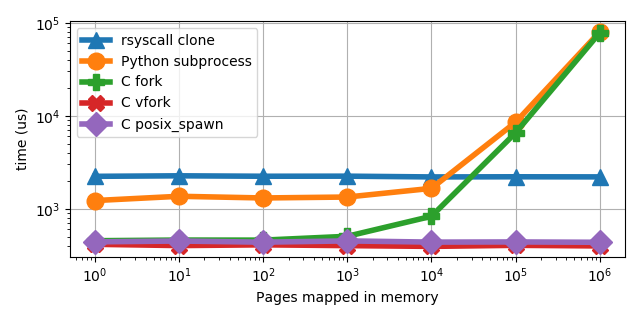
\includegraphics[width=0.5\textwidth]{subprocess_bench}
 \caption{Python spawn-style vs direct-style performance under varying memory usage}
 \label{fig:subprocess_bench}
\end{figure}
In Python, does our \texttt{rsyscall}-based direct-style process creation interface
have acceptable performance relative to the standard library's spawn-style \texttt{subprocess.run}?

We first evaluate a simple process creation workload:
create a child process, exec the \texttt{true} binary, and wait for it to exit.
We implement this using both direct-style \texttt{clone}
and the standard library's \texttt{subprocess.run}.
We benchmark both implementations under CPython 3.7.7, on Linux 4.19.93,
pinned to an isolated single core on an Intel i9-9900K CPU with 60GB of RAM.
We vary the amount of anonymous memory mapped in the parent process
to demonstrate how each implementation scales with memory usage.
The results are in Figure \ref{fig:subprocess_bench}.

The direct-style implementation stays around 2.2 milliseconds regardless of memory usage.
\texttt{subprocess.run}, which is implemented with \texttt{fork},
starts at 1.4 milliseconds,
and then scales linearly with the amount of memory mapped, as expected,
up to 48.5 milliseconds at 4 GBs of mapped memory.
The cross-over point for this micro-benchmark is about 40 megabytes of memory mapped.

We perform another microbenchmark to evaluate the overhead of modifying the child process.
We simply call \texttt{getpid} from Python
in both the child process and the parent process on the same benchmark setup.
The average time per \texttt{getpid} call is
3 microseconds when called in the parent process without going through \texttt{rsyscall},
and 561 miroseconds when called through \texttt{rsyscall} in the child process.
The difference, 558 microseconds,
is the amount of overhead incurred
by performing our child process setup system calls through \texttt{rsyscall}.
Through profiling, we've found that most of this per-syscall overhead is spent in Python,
rather than waiting for syscall responses from the child task.

These slowdowns in process creation and modification are substantial,
but we found that this overhead is acceptable in practice.
Process creation in Python is already slow, taking milliseconds of time,
so it is not expected to be on the fast path.
In that context, \texttt{rsyscall} has a reasonable cost compared to \texttt{subprocess.run},
and avoids the bad scaling of \texttt{fork} which might be unexpected by the naive programmer.

Furthermore, as we'll discuss in section \ref{realworld},
we've found that the greater expressivity of direct-style
provides for programs that are more efficient on a large scale,
which makes up for the performance cost in micro-benchmarks.
We've also found that, for many interesting applications,
the performance overhead of direct-style process creation (or Python, for that matter)
is dwarfed by the execution time of the native-code programs we ultimately run.

As a result, though implementations in native code and in the kernel would likely remove most of this overhead,
we have chosen to not invest effort into optimizing process creation at this micro-level,
to preserve implementation simplicity;
such optimization is reserved for future work.
\subsection{Usage in the real world}\label{realworld}
At \twosigma we have used \texttt{rsyscall} and direct-style process creation
as a component of an internal distributed system deployment library, written in Python.
This library is in use in production,
and is extensively used as part of testing and development.

Each service deployed by this library is started with custom code,
written using direct-style process creation.
This allows us to pass down file descriptors and initialize process attributes
according to each program's needs;
which in turn has let us make optimizations which previously required too much program-specific customization.

For example,
we are able to bootstrap connections over our internal shared memory transports over passed-down file descriptors,
and our management interfaces listen on passed-down sockets.
This allows substantial parallelism in the startup of services.\cite{socketactivation}
Taking one representative example,
one test built with an old library took an average of 221 seconds to run,
mostly spent in system startup time as processes started up serially.
With parallelized system startup, the same test takes an average of 16 seconds.

We've found that programmers
are able to use file descriptor passing as a normal feature of their development process with relative ease.
Programmers without substantial prior experience with Unix programming
are able to write code to support new services
nd pass down file descriptors to the program without encountering significant issues.

We also flexibly use namespaces where appropriate.
For example, for legacy applications which directly start subprocesses,
we prevent process leaking with a pid namespace.

All this has allowed us to run our systems in a much more dynamic way than before.
We can freely start up arbitrary subsets of our systems on-demand,
spread across one or more hosts,
for development, testing, or production,
regardless of the configuration of that host,
without worrying about interference between instances,
and without a dependency on any external privileged services,
such as container runtimes.
This has become a key part of our development workflow.
\section{Related work}\label{related_work}
\subsection{Direct-style process creation}
Baumann 2019\cite{forkroad} briefly suggests cross-process operations as a possible replacement for fork on Unix,
positing many of the same advantages we find in practice.
Our work, though developed independently,
is in many ways an elaboration on and implementation of that idea,
to which we owe a great debt.

As we discuss in section \ref{background},
many academic operating systems have direct-style process creation.
We are not aware of any previous instances of direct-style process creation in a Unix-like environment.

The closest related work known to us
is efforts to build Unix compatibility environments, including fork-style process creation,
on academic operating systems which natively use direct-style process creation.\cite{exokernel}
Such compatibility environments could theoretically be bypassed to perform direct-style process creation
using the underlying primitives,
but regular Unix system calls could not be used to create new Unix processes in a direct-style way
in such an environment.
\subsection{Remote system calls}
There are many Unix-based systems which do something called "remote system calls".
Most such systems do not allow a single program to manipulate multiple processes.
Those systems that do allow manipulating multiple processes
are generally oriented towards debugging and introspection,
and are unsuitable for a general purpose system.

Many systems use system call forwarding to implement migration in a computing cluster.
HTCondor\cite{condor} and Popcorn\cite{popcorn} are two examples.
In both systems, processes can be live-migrated between hosts;
when this occurs, the system will automatically forward IO-related system calls
back to the original host.

Some systems intercept system calls and forward them to another process to be implemented
as part of a virtualization system.
gvisor\cite{gvisor} and ViewOS\cite{viewos} are two examples.
In both systems,
system calls made in one process are intercepted,
and serviced by another process.

Some systems forward system calls elsewhere for asynchronous execution.
FlexSC\cite{flexsc} is one example.
System calls in FlexSC are forwarded to a pool of dedicated system call execution threads.
The recently added Linux feature \verb|io_uring| is, in some sense, another example;
it supports sending a subset of system calls to the kernel,
which executes them asynchronously,
rather than blocking the thread.

Some systems call system calls in other processes for debugging or introspection purposes.
strace, gdb, and CRIU\cite{criu} are examples of this.
These systems typically uses ptrace,
which is capable of operating on multiple processes at once.
As discussed in section \ref{implementation},
a ptrace-based has approach has limitations which make it unsuitable for \texttt{rsyscall}.
\subsection{Process capabilities}
The Capsicum system provides something called process descriptors\cite{capsicum},
which is a file descriptor handle for a process.
A similar feature has been recently added to Linux in the form of the pidfd API\cite{pidfd}.
These notions of process capability are quite limited, however;
pidfds and process descriptors only allow sending signals to a process or waiting for its death,
rather than exercising full control over the process.
\subsection{Capability-secure libc replacements}
The Capsicum system provides a set of system calls
which can be used to provide a capability-secure sandbox.\cite{capsicum}
Latter efforts\cite{oblivious}, including CloudABI\cite{cloudabi} and WASI\cite{wasi},
developed this into a partial or full replacement for a POSIX libc.
Like all other Unix libcs that we know of,
these libc-replacements implicitly make system calls on the current process,
rather than using an explicit process capability as \texttt{rsyscall} does.

PLASH provides a spawn-style API, in the form of a shell,
to launch processes in a capability-secure environment.\cite{plash}
PLASH, like all spawn-style APIs, abstracts over the native Linux environment,
and is therefore limited in what kind of processes it can create.
\section{Future work}\label{future_work}
\subsection{Other applications of \texttt{rsyscall}}
Most avenues of future work focus on \texttt{rsyscall}.
\texttt{rsyscall} was not developed solely for the purpose of this paper,
and it has other uses unrelated to direct-style process creation,
such as asynchronous system calls, exceptionless system calls\cite{flexsc}, cross-host operations, among others.
We are actively exploring such applications,
as well as broadening \texttt{rsyscall}'s language support.
\subsection{Kernel support}
\texttt{rsyscall}'s cross-process syscalls can be performed entirely in userspace,
which has substantial benefits for deployability.
Nevertheless, direct support in the Linux kernel
for creating a stub process and performing syscalls in the context of that process
may provide efficiency benefits, as well as reducing userspace-visible complexity.

Several other aspects of our implementation would also be improved by new features in the Linux kernel,
as discussed in sections \ref{execve} and \ref{cloexec}.
\subsection{Portability to other Unix systems}
Other non-Linux systems
could adopt the techniques of this paper
to provide direct-style process creation.
Currently, our focus is on Linux,
but others may wish to explore porting these techniques to other operating systems.
% TODO maybe we could get rid of this paragraph?
\subsection{Large scale open source usage}
We would like to open source libraries built on top of direct-style process creation.
From our experience using such libraries at \twosigma,
we believe this would greatly ease the development of complex systems involving processes,
and would provide a substantial demonstration of the power of direct-style process creation.
\section{Conclusions}\label{conclusions}
Direct-style process creation is much less known and much less used than fork-style and spawn-style.
We have implemented direct-style process creation for Linux.
Our implementation is immediately deployable on today's Linux systems.
We have discussed various applications of processes,
and demonstrated the use of Linux direct-style process creation
to implement them.

We believe that direct-style process creation is superior to fork-style and spawn-style,
including on Linux.
Our technique is immediately deployable and can be used for a wide variety of complex applications.

We hope that a better process creation mechanism
will help encourage more creative use of processes,
which, though widespread,
are still not used to their full potential.

\bibliographystyle{plain}
\bibliography{bibliography}
\end{document}
